\documentclass[reducespace,stylepage,semiarbeit]{spezidoc}
\usepackage[ngerman]{babel}
\usepackage{graphicx}
\usepackage{amssymb}
\usepackage{amsfonts}
\interfootnotelinepenalty=10000



\schuelerone{Lukas}{Schneider}{12as}
\schuelertwo{Moritz}{Vogel}{12bs}
\schuelerthree{Joris}{Kühl}{12as}
\seminarfachbetreuer[true]{Frau Doktor Marion Moor}
\fachbetreuerone[false]{Herr Bodo Gramsch}
\aussenbetreuer[false]{Herr Doktor Florian Römer}
\title{Simulation Ultraschall-basierter zerstörungsfreier Materialprüfung}
\date{\today}
\parindent0pt
\setlength{\parskip}{\baselineskip}
\usepackage[ngerman]{babel}
\usepackage{graphicx}
%\usepackage{subcaption}
%\usepackage{caption}
%\usepackage{setspace}
%\usepackage{ulem}
%\usepackage{wrapfig}
\usepackage[style=science, backend=bibtex]{biblatex} %style=verbose
\bibliography{Theorie_Ultraschall}

\begin{document}
\maketitlepage
\newpage
\tableofcontents
\thispagestyle{empty}
\newpage

\setcounter{page}{1}

\section{Theorie der Zerstörungsfreien Prüfung}
\subsection{Definition zerstörungsfreier Prüfung}
Das Gebiet der Material- oder Werkstoffprüfung befasst sich mit der Ermittlung der Kenngrößen und des Verhaltens fertiger Bauteile, z.B. einer Eisenbahnschiene, und Werkstoffproben, etwa eines Steinblocks. Getestet werden können zum Beispiel Dehnbarkeit, Hitzebeständigkeit oder Fehlerfreiheit.\\ 
%[https://de.wikipedia.org/wiki/Werkstoffpr%C3%BCfung]
Unter Fehlern versteht man dabei Unregelmäßigkeiten beziehungsweise Abweichungen von der Norm an der Oberfläche oder im Inneren des Bauteils oder Werkstoffs (Im Weiteren Prüfkörper), welche die Verwendbarkeit desselben beeinträchtigen. 
Man unterscheidet weiterhin bei der Werkstoffprüfung zwischen zerstörenden und zerstörungsfreien Verfahren. Zu ersterer Kategorie zählen unter anderem Stresstests, bei denen die Grenzen eines Prüflings getestet werden. Ein Test der Reißfestigkeit eines Seils etwa ist dann beendet, wenn es reißt. Mit ähnlichen Verfahren lassen sich viele Informationen ermitteln und die zerstörenden Verfahren decken ein entsprechend breites Spektrum ab. Sie versagen allerdings in einem sehr wichtigen Anwendungsgebiet der Materialprüfung - der Fehlerprüfung.\\
Anders als die Ermittlung allgemeiner Informationen über ein Produkt müssen Fehlerprüfungen regelmäßig durchgeführt werden. Man nehme zum Beispiel eine Halterung für Flugzeugturbinen. Die Belastbarkeit des Bauteils ist hier eine entscheidende Information und wird daher genau (zerstörend) gemessen, was zur Zerstörung des Bauteils führt. Wenn man einige Bauteile verwendet um den Test durchzuführen und starke Abweichungen streicht erhält man sehr wahrscheinlich einen Wert, der die zu erwartende Belastbarkeit des Bauteils widerspiegelt und Kunden zur Information dienen kann. Die dabei zerstörte Menge an Halterungen ist ein vernachlässigbarer Verlust.\\
Möchte man jedoch wissen, wie die weiteren produzierten Bauteile beschaffen sind, muss man nicht mehr den genauen Wert ermitteln, sondern nur auf Abweichungen von der Norm prüfen, also auf Fehler. Ein naheliegender Einfall ist, Stichproben zu nehmen, was jedoch zwei Nachteile hat: Zum einen ist selbst der Verlust einzelner Teile ein Verlust, und damit nicht wünschenswert. Zum anderen ist eine Stichprobe nicht sicher, da diese nur zuverlässige Fehler, hervorgerufen durch eine dauerhafte Fehlfunktion in der Fertigung, eindeutig feststellt.\\
Beide Probleme werden durch zerstörungsfreie Materialprüfung gelöst. Wie der Name schon sagt, wird der Prüfkörper bei diesen Verfahren nicht verbraucht, was diverse Vorteile hat. So kann man nun alle Bauteile prüfen und dennoch verkaufen. Diese Prüfverfahren eignen sich auch für eine Prüfung lange nach der Fertigung, bei der festgestellt werden soll, ob durch den Gebrauch Fehler entstanden sind. Hier wäre eine Stichprobe gänzlich nutzlos und eine vollständige Zerstörung ginge gegen den Sinn der Prüfung. Zerstörungsfreie Verfahren dagegen ermöglichen es, festzustellen, ob Teile ersetzt werden müssen und falls nicht, fallen nur die Kosten für die eigentliche Prüfung an.\\
Ein Nachteil dieser Methoden ist jedoch, dass sie nur auf Fehler aufmerksam machen, anstatt ihre Wirkung einzuschätzen. Die Ablösung der zerstörenden Prüfung auf dem Gebiet der Bestimmung von Kenngrößen ist also zumindest mit den momentan bekannten Methoden der zerstörungsfreien Prüfung noch nicht möglich.
\newpage

\subsection{Ultraschall-basierte Werkstoffprüfung}
Eines der wichtigsten Verfahren im Bereich der zerstörungsfreien Prüfung ist die Ultraschall-Fehlerprüfung. Es basiert darauf, dass Schallwellen von einem Prüfkopf aus in einen Probekörper eingeleitet und anschließend eventuelle Reflexionen gemessen werden. Diese Messungen werden dann in einem sogenannten Oszillogramm dargestellt.
%\begin{figure}[h]\begin{center}
%\label{oszillogramme}
%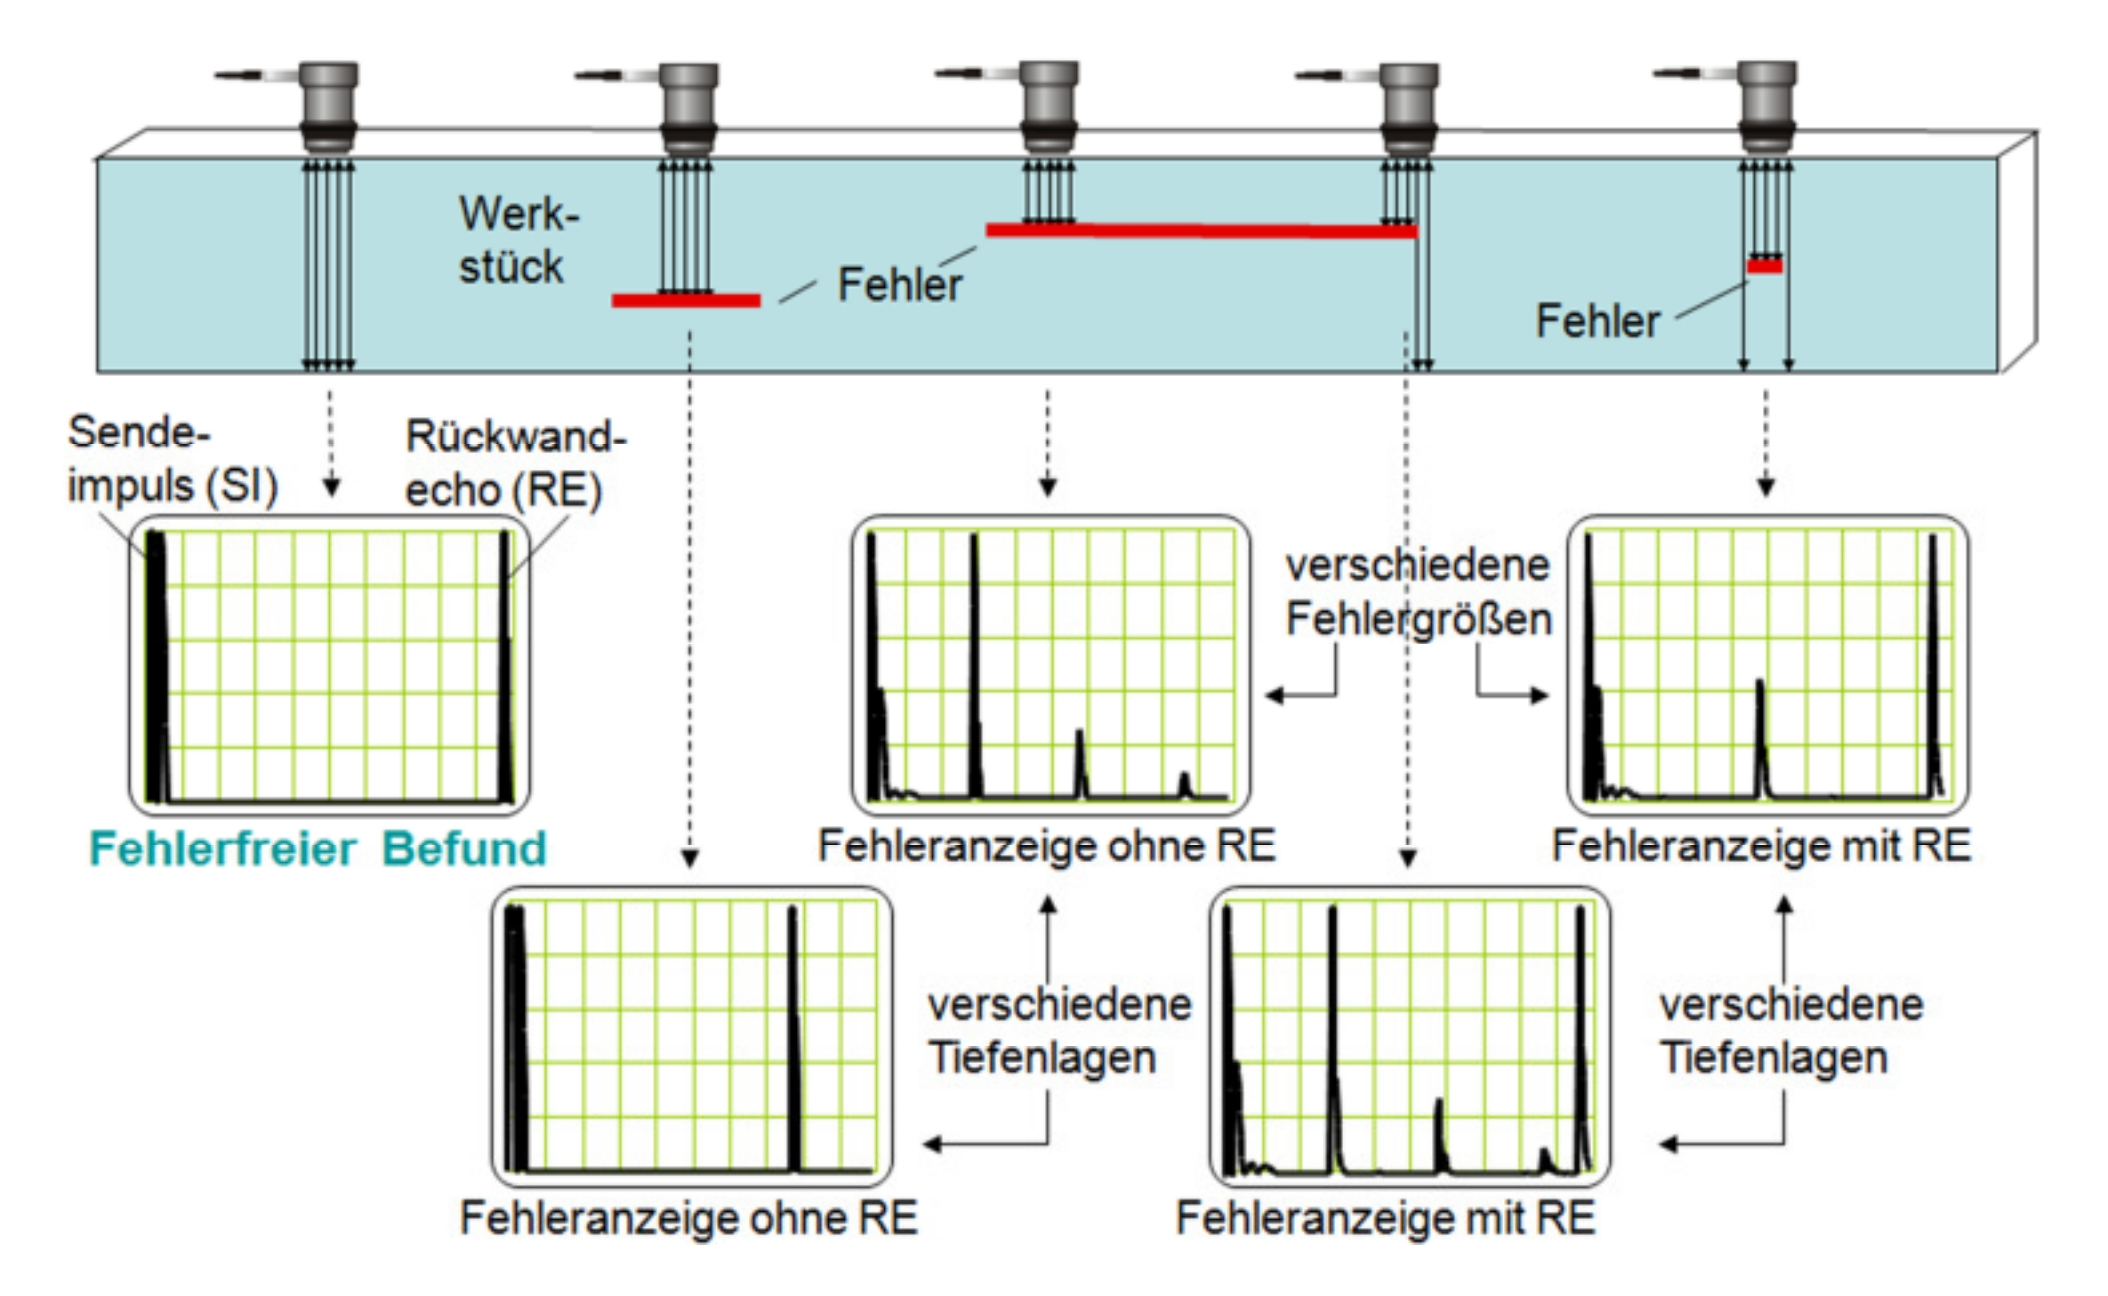
\includegraphics[width=.85\textwidth]{Oszillogramme.jpg}
%\caption{Oszillogramme (beispielhaft, Nummer eins bis fünf von links nach rechts)}
%\end{center}\end{figure}\\
Je höher dabei eine Spitze (auch Peak) ist, desto stärker war das zugehörige Echo. Hierbei wird ausgenutzt, dass beim Übergang der Ultraschallwellen von einem Material zum anderen ein bestimmter Anteil reflektiert wird, während ein anderer Anteil (unter einem anderen Winkel) sich weiter durch den Körper bewegt. Trifft eine Schallwelle, die sich in einem festen Körper bewegt, auf Luft, so wird sie beinahe vollständig zurückgeworfen, weshalb etwaige passierende Schallwellen gering genug sind, um vernachlässigt werden zu können. So erscheint das erste Echo schon direkt zu Beginn der Messung, wie im ersten Oszillogramm zu sehen: es entsteht, wenn die ausgesandten Wellen in den Probekörper eintreten, denn zwischen Prüfkopf und Probekörper befindet sich immer eine (meist sehr dünne) Luftschicht; daher wird der Schall schon einmal reflektiert, bevor der relevante Teil des Verfahrens beginnt. Um dies in der Praxis zu minimieren, wird eine Kopplungsflüssigkeit verwendet, welche den Schall mit möglichst wenig Reflexionen zwischen Werkstück und Prüfkopf transportiert. Das zweite Echo stellt in diesem Fall das sogenannte Rückwandecho dar, bei welchem die Wellen von der dem Prüfkopf gegenüberliegenden Seite zurückgeworfen werden. Mithilfe dessen kann auch Tiefe des Probekörpers ermittelt werden: da der Schall stets eine materialspezifische Geschwindigkeit $c_\mathrm{Material}$ \cite{schallgeschwindigkeiten} besitzt, gilt für die Stärke des Körpers: $d = \dfrac{c_\mathrm{Material}~\cdot~t}{2}$. Dies ist vor allem hilfreich, wenn Probeköper nur von einer Seite erreichbar sind und ihre Dimensionen daher nicht mit herkömmlichen Werkzeugen bestimmt werden können.\\
Für die zerstörungsfreie Prüfung ist diese Möglichkeit jedoch eher von geringerer Bedeutung. Der eigentliche Nutzen von Ultraschall lässt sich besser an den anderen Oszillogrammen erklären. Befinden sich Fehler im Werkstück, sind das meist Lufteinschlüsse in Form von Rissen oder Löchern. Da sich somit auch dort ein Materialübergang befindet, werden Schallwellen an Fehlstellen ebenfalls reflektiert. Analog zur Bestimmung der Maße des Körpers können auch die ungefähren Positionen der Fehler ermittelt werden. Der große Vorteil dieses Verfahrens ist, dass es nahezu unbegrenzt einsetzbar ist, da sich Sender und Empfänger in einem Gerät befinden und so auch bei komplexen Geometrien, welche nur eingeschränkt zugänglich sind, genutzt werden können. Problematisch ist hingegen die Auswertung der entstehenden Oszillogramme. Zum Beispiel Oszillogramm Nummer vier: einerseits gibt es das normale Rückwandecho, also befindet sich der Prüfkopf teilweise über einem Streifen ohne Fehler; zusätzlich existieren jedoch noch weitere Echos, die auf Fehlstellen hinweisen. Eine mögliche Deutung wäre, dass es mehrere verschieden große Lufteinschlüsse in unterschiedlichen Tiefen gibt, welche die Echos verursachen. Diese Interpretation wäre allerdings falsch, denn wie man sehen kann, gibt es nur einen Fehler, von dem das Echo immer wieder reflektiert wird. An dieser Stelle muss man anmerken, dass in diesem Fall kein gutes Kopplungsmittel verwendet wurde, da sonst das Echo sehr viel schneller abschwächen würde. Der Grund dafür, dass es dennoch schwächer wird, ist einerseits der Fakt, dass die Wellen teilweise die Fehlstelle passieren und somit ein wenig ihrer Stärke verlieren, andererseits aber auch die Streuung der Schallwellen im Körper, sodass das Signal stetig schwächer wird.\\
Im Detail kann die Verfahrensweise der zerstörungsfreien Materialprüfung mit Ultraschall nachgelesen werden in Quelle \cite{karldeutsch}.
\end{document}